\def\foo{\vphantom{fy}}
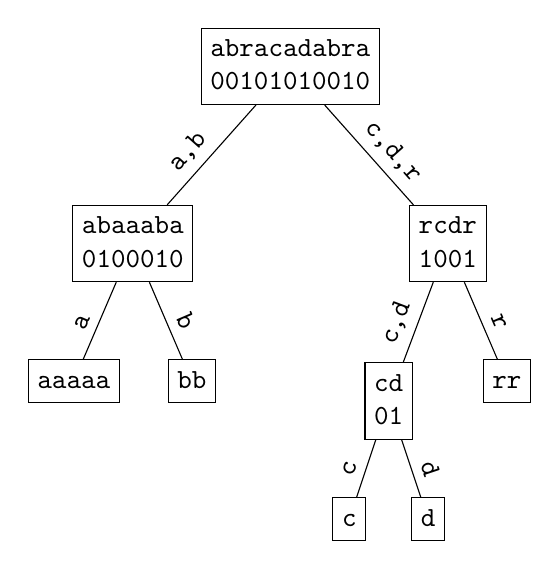
\begin{tikzpicture}[every text node part/.style={align=center}]
  \node[draw] (0) at (0,0) {\texttt{abracadabra}\foo\\\texttt{00101010010}\foo};
  \node[draw] (1) at (-2,-2.25) {\texttt{abaaaba}\foo\\\texttt{0100010}\foo};
  \node[draw] (2) at (-2.75,-4) {\texttt{aaaaa}\foo};
  \node[draw] (3) at (-1.25,-4) {\texttt{bb}\foo};
  \node[draw] (4) at (2,-2.25) {\texttt{rcdr}\foo\\\texttt{1001}\foo};
  \node[draw] (5) at (1.25,-4.25) {\texttt{cd}\foo\\\texttt{01}\foo};
  \node[draw] (6) at (0.75,-5.75) {\texttt{c}\foo};
  \node[draw] (7) at (1.75,-5.75) {\texttt{d}\foo};
  \node[draw] (8) at (2.75,-4) {\texttt{rr}\foo};

  \draw (0) -- (1) node [above,sloped,pos=0.6] {\texttt{a,b}};
  \draw (1) -- (2) node [above,sloped,pos=0.6] {\texttt{a}};
  \draw (1) -- (3) node [above,sloped,pos=0.6] {\texttt{b}};
  \draw (0) -- (4) node [above,sloped,pos=0.6] {\texttt{c,d,r}};
  \draw (4) -- (5) node [above,sloped,pos=0.6] {\texttt{c,d}};
  \draw (4) -- (8) node [above,sloped,pos=0.6] {\texttt{r}};
  \draw (5) -- (6) node [above,sloped,pos=0.6] {\texttt{c}};
  \draw (5) -- (7) node [above,sloped,pos=0.6] {\texttt{d}};
\end{tikzpicture}
